\documentclass[11pt]{article}
\usepackage{mathtools}
\usepackage{amssymb}
\usepackage{amsthm}
\usepackage{polski}
\usepackage[utf8]{inputenc}
\usepackage{geometry}
\usepackage{mnsymbol}
\usepackage{graphicx}
\usepackage{textgreek}
\usepackage{float}
\usepackage{caption}
\author{Łukasz Jezapkowicz}
\title{Diody Półprzewodnikowe}
\date{3.05.2019}
\begin{document}
\newgeometry{tmargin=2cm,bmargin=2cm,lmargin=2cm,rmargin=2cm}
\maketitle
\tableofcontents \newpage
\section{Działanie prostownicze diody półprzewodnikowej w obwodzie elektrycznym}
\subsection{Cel ćwiczenia}
Celem ćwiczenia było zapoznanie się z prostym obwodem elektrycznym z diodą oraz zmierzenie napięcia progowego diody półprzewodnikowej przy pomocy oscyloskopu i analizy Transient.
\subsection{Przebieg ćwiczenia}
Na pulpicie symulacyjnym zbudowałem obwód elektryczny widoczny na \textbf{Rys. 1}. Przedstawiony poniżej układ zawiera źródło napięcia zmiennego $V_1$ o wartości $10V$ i częstotliwości $1kHz$, rezystor $R_1$ o oporze równym $1k\Omega$ oraz diodę półprzewodnikową $D_1$.
W celu zbadania napięcia progowego dołączyłem do obwodu oscyloskop $XSC1$.
\begin{figure}[H]
\centering
\includegraphics[width=10cm]1
\caption*{\textbf{Rys. 1}: Schemat obwodu elektrycznego z diodą i dołączonym oscyloskopem.}
\end{figure}
\noindent W celu obliczenia napięcia progowego skorzystam z oscyloskopu a później z analizy Transient i porównam wyniki. By obliczyć napięcie progowe odczytuję różnicę największego napięcia $V_1$ i największego napięcia $V_2: V_P = V_1MAX - V_2MAX = 14.111 V - 13.421 V = 0.69 V$. 
Odczytane napięcia widać na \textbf{Rys. 2} poniżej.
\begin{figure}[H]
\centering
\includegraphics[width=10cm]2
\caption*{\textbf{Rys. 2}: Ekran oscyloskopu dołączonego do układu z diodą półprzewodnikową.}
\end{figure}
\noindent Teraz zrobię to samo tylko przy pomocy analizy Transient. Wyniki analizy widać na \textbf{Rys. 3}. Po odczytaniu największego napięcia $V_1$ i $V_2 : V_P = V_1MAX - V_2MAX = 14.0801 V - 13.3906 V = 0.6895 V$.
\begin{figure}[H]
\centering
\includegraphics[width=10cm]3
\caption*{\textbf{Rys. 3}: Analiza Transient układu z diodą półprzewodnikową.}
\end{figure}
\noindent Na koniec zmierzyłem napięcie średnie $U_{śr}$. W tym celu dołączyłem do układu multimetr $XMM2$ i multimetr agilent $XMM3$. Zmierzone wartości widać na \textbf{Rys. 4}.
\begin{figure}[H]
\centering
\includegraphics[width=10cm]4
\caption*{\textbf{Rys. 4}: Układ z dołączonym multimetrem i multimetr agilent.}
\end{figure}
\noindent Wyniki moich działań podsumowałem w tabelce widocznej na \textbf{Rys. 5}. W tabelce widać również wyniki dla diody podłączonej w kierunku zaporowym.
\begin{figure}[H]
\centering
\includegraphics[width=10cm]5
\caption*{\textbf{Rys. 5}: Tabela podsumowująca wyniki ćwiczenia.}
\end{figure}
\subsection{Wnioski}
Ćwiczenie pokazuje, że zmierzenie napięcia progowego diody półprzewodnikowej to rzecz szybka i łatwa. Jak widać w tabelce na \textbf{Rys. 5} wyniki w analizie Transient i na ekranie oscyloskopu zgadzają się. Napięcie średnie w obwodzie wynosi ok. $4.17 V$. Zmierzona wartość napięcia progowego jest bliska rzeczywistości. Wykonane ćwiczenie potwierdza
występowanie napięcia progowego w diodzie półprzewodnikowej.
\section{Prostownik jednopołówkowy z filtrem RC na wyjściu}
\subsection{Cel ćwiczenia}
Celem ćwiczenia było zapoznanie się z prostym układem elektrycznym z prostownikiem jednopołówkowym z filtrem RC oraz wielokrotne zmierzenie napięcia tętnień przy podanych parametrach układu.
\subsection{Przebieg ćwiczenia}
Na pulpicie symulacyjnym zbudowałem obwód elektryczny widoczny na \textbf{Rys. 6}. Przedstawiony poniżej układ zawiera źródło napięcia zmiennego $V_1$ o wartości $10V$ i częstotliwości $1kHz$, diodę półprzewodnikową $D_1$, kondensator $C_1 = 2\mu$$F$, rezystor $R_1 = 1k\Omega$ oraz transformator.
Do układu podłączyłem również oscyloskop w celu zbadania napięcia tętnień.
\begin{figure}[H]
\centering
\includegraphics[width=10cm]6
\caption*{\textbf{Rys. 6}: Schemat obwodu elektrycznego z transformatorem i diodą półprzewodnikową. Układ zawiera również dołączony oscyloskop.}
\end{figure}
\noindent Do obliczenia napięcia tętnień posłużyłem się analizą Transient. Jej wyniki dla obwodu przedstawionego powyżej widoczne są na \textbf{Rys. 7}. Napięcie tętnień obliczyłem jako różnicę największego napięcia i najmniejszego napięcia za diodą$: U_T = U_{MAX} - U_{MIN} = 13.4063 V - 8.8078 V = 4.5985 V$.
\begin{figure}[H]
\centering
\includegraphics[width=10cm]8
\caption*{\textbf{Rys. 7}: Analiza Transient dla obwodu elektrycznego z Rys. 6}
\end{figure}
\noindent W celu sprawdzenia poprawności obliczonego wyniku obliczyłem również napięcie tętnień dla układu z \textbf{Rys. 6} za pomocą oscyloskopu. Ekran oscyloskopu widać na \textbf{Rys.8}. Napięcie obliczyłem w taki sam sposób$: U_T = U_{MAX} - U_{MIN} = 13.428 V - 8.832 V = 4.596 V$.
\begin{figure}[H]
\centering
\includegraphics[width=10cm]7
\caption*{\textbf{Rys. 8}: Ekran oscyloskopu podłączonego do obwodu elektrycznego z Rys. 6}
\end{figure}
\noindent Pomiary wykonałem również przy trzech innych sytuacjach: bez kondensatora w obwodzie, z kondensatorem o pojemności $1\mu$$F$ oraz z kondensatorem o takiej pojemności by napięcie tętnień stanowiło 10 procent wartości maksymalnej napięcia. Taką pojemnością okazało się $8\mu$$F$. Wyniki wszystkich pomiarów 
wpisałem do tabelki widocznej na \textbf{Rys. 9}.
\begin{figure}[H]
\centering
\includegraphics[width=10cm]9
\caption*{\textbf{Rys. 9}: Tabelka z wynikami pomiarów z róznymi pojemnościami kondensatorów. }
\end{figure}
\subsection{Wnioski}
Z powyższej tabelki widać, że po dodaniu kondensatora pojawia się napięcie tętnień będące skutkiem ładowania i rozładowywania kondensatora. Im większa pojemność kondensatora tym mniejsze napięcia tętnień. Wynika to z tego, że kondensator zbiera wtedy większy ładunek. Wraz ze wzrostem rezystancji tętnienia 
również maleją co wynika z mniejszego prądu w układzie (kondensator wolniej się rozładowuje). Dla oporu $R_1 = 1k\Omega$ i pojemności kondensatora $C_3 = 8\mu$$F$ napięcia tętnień wynoszą ok. 10 procent wartości maksymalnej.
\section{Prostownik w układzie Graetza}
\subsection{Cel ćwiczenia}
Celem ćwiczenia było zapoznanie się z prostym układem elektrycznym z prostownikiem dwupołówkowym (mostkiem Graetza) oraz wielokrotne zmierzenie napięcia tętnień przy podanych parametrach układu.
\subsection{Przebieg ćwiczenia}
Na pulpicie symulacyjnym zbudowałem obwód elektryczny widoczny na \textbf{Rys. 10}. Przedstawiony poniżej układ zawiera źródło napięcia zmiennego  $V_1$ o wartości $10V$ i częstotliwości $1kHz$, 4 diody półprzewodnikowe tworzące mostek Graetza, kondensator $C_1 = 5\mu$$F$, rezystor $R_1 = 1k\Omega$ oraz transformator. Do układu podłączyłem również oscyloskop w celu zbadania napięcia tętnień.
\begin{figure}[H]
\centering
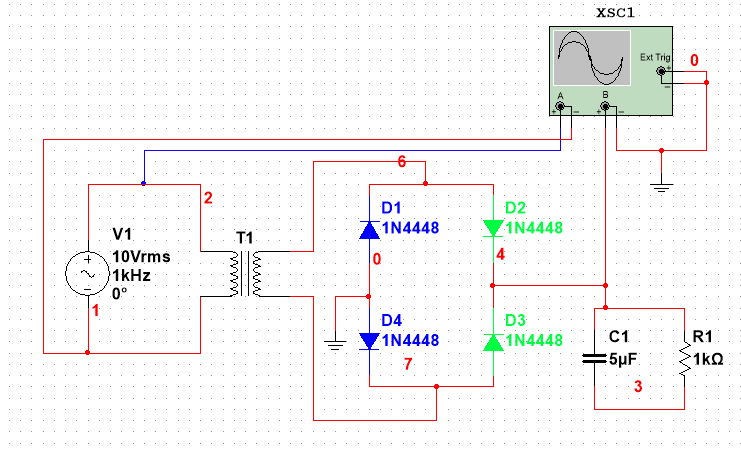
\includegraphics[width=10cm]{10}
\caption*{\textbf{Rys. 10}: Schemat obwodu elektrycznego z transformatorem i mostkiem Graetza. Układ zawiera również dołączony oscyloskop.}
\end{figure}
\noindent Do obliczenia napięcia tętnień posłuzyłem się analizą Transient. Jej wyniki dla obowdu przedstawionego na \textbf{Rys. 10} widoczne są na \textbf{Rys. 11}. Napięcie tętnień obliczyłem jako różnicę największego napięcia i najmniejszego napięcia wyjścia$: U_T = U_{MAX} - U_{MIN} = 12.6072 V - 11.6485 V = 0.9587 V $.
\begin{figure}[H]
\centering
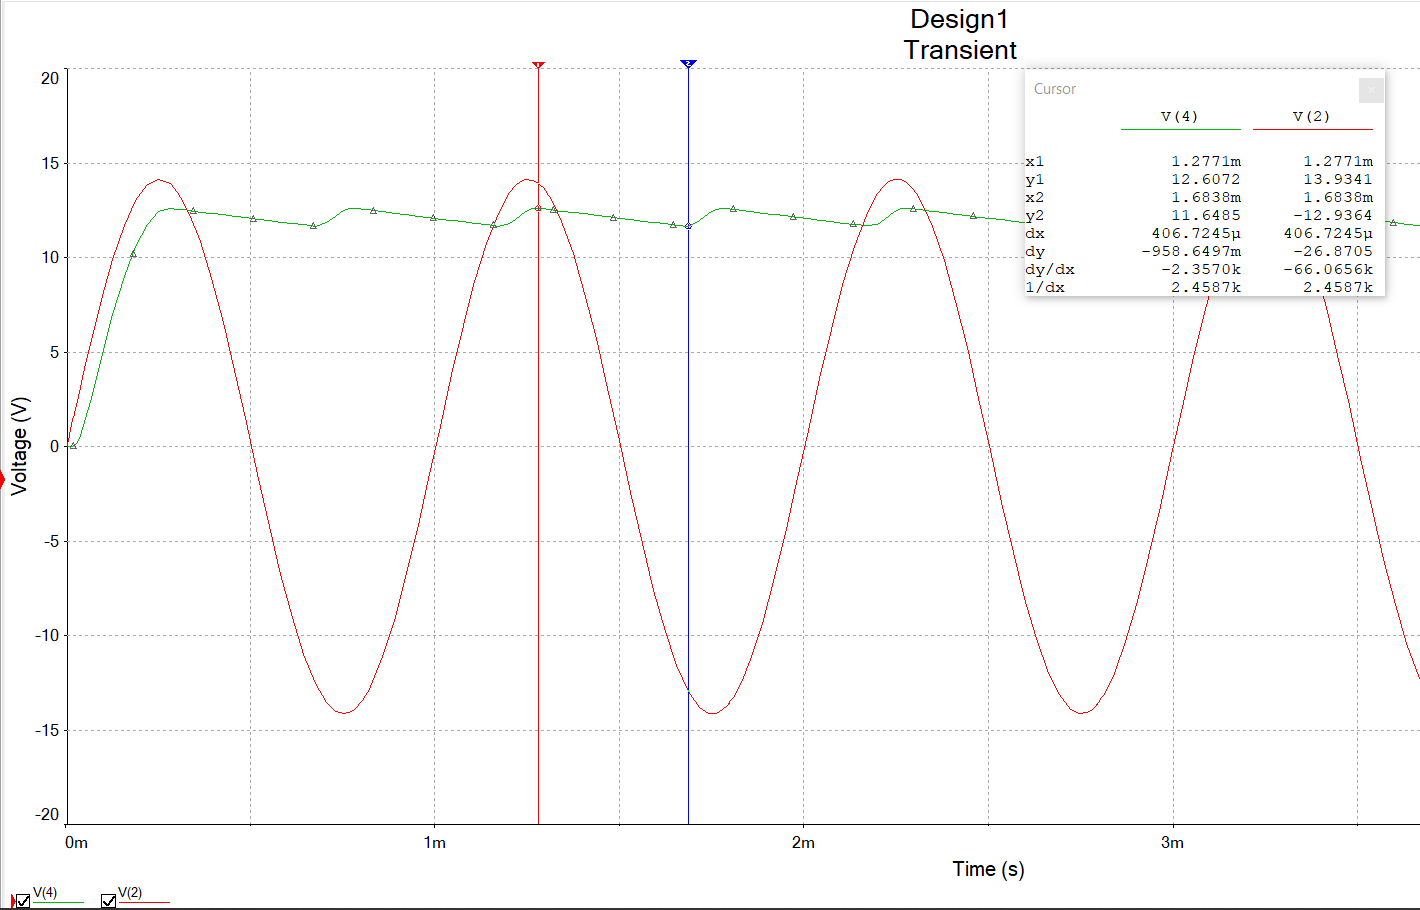
\includegraphics[width=10cm]{12}
\caption*{\textbf{Rys. 11}: Analiza Transient dla obwodu elektrycznego z Rys. 10}
\end{figure}
\noindent W celu sprawdzenia poprawności obliczonego wyniku obliczyłem również napięcie tętnień dla układu z \textbf{Rys. 6} za pomocą oscyloskopu. Ekran oscyloskopu widać na \textbf{Rys.8}. Napięcie obliczyłem w taki sam sposób$: U_T = U_{MAX} - U_{MIN} = 12.596 V - 11.706 V =  0.890 V$.
\begin{figure}[H]
\centering
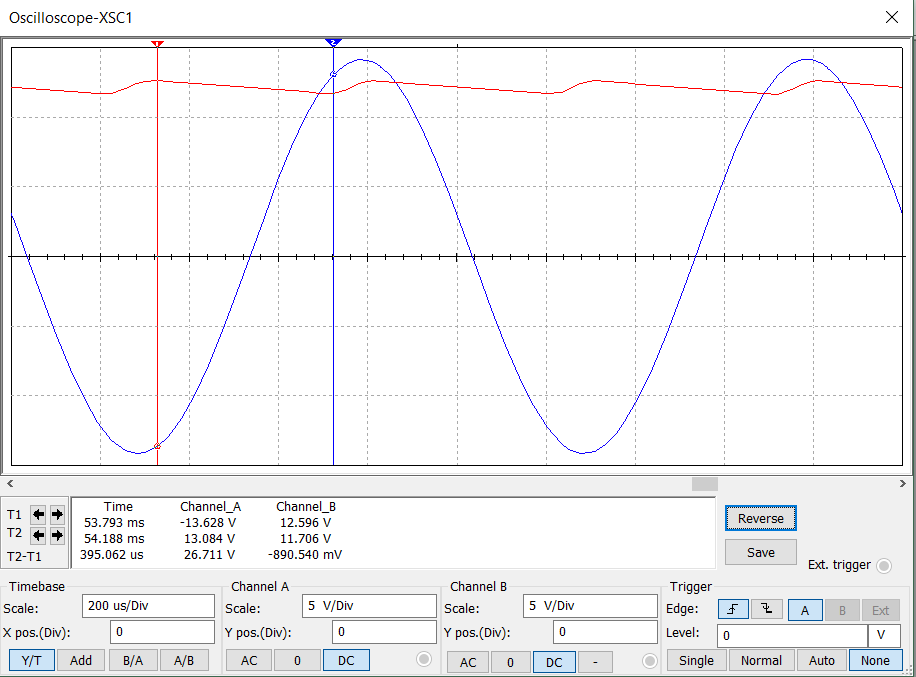
\includegraphics[width=10cm]{11}
\caption*{\textbf{Rys. 12}: Ekran oscyloskopu podłączonego do obwodu elektrycznego z Rys. 10}
\end{figure}
\noindent Pomiary wykonałem również przy trzech innych sytuacjach: bez kondensatora w obwodzie, z kondensatorem o pojemności $5\mu$$F$ i oporem $R_1 = 10k\Omega$ oraz z kondensatorem o takiej pojemności by napięcie tętnień stanowiło 10 procent wartości maksymalnej napięcia. Taką pojemnością okazało się $3.8\mu$$F$. Wyniki wszystkich pomiarów wpisałem do tabelki widocznej na \textbf{Rys. 13}.
\begin{figure}[H]
\centering
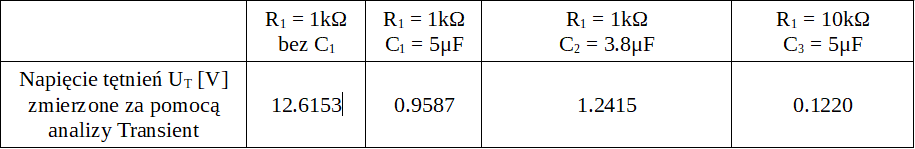
\includegraphics[width=10cm]{13}
\caption*{\textbf{Rys. 13}: Tabelka z wynikami pomiarów z róznymi pojemnościami kondensatorów. }
\end{figure}
\noindent Przeanalizowałem również trzy możliwe uszkodzenia układu.
\begin{figure}[H]
\centering
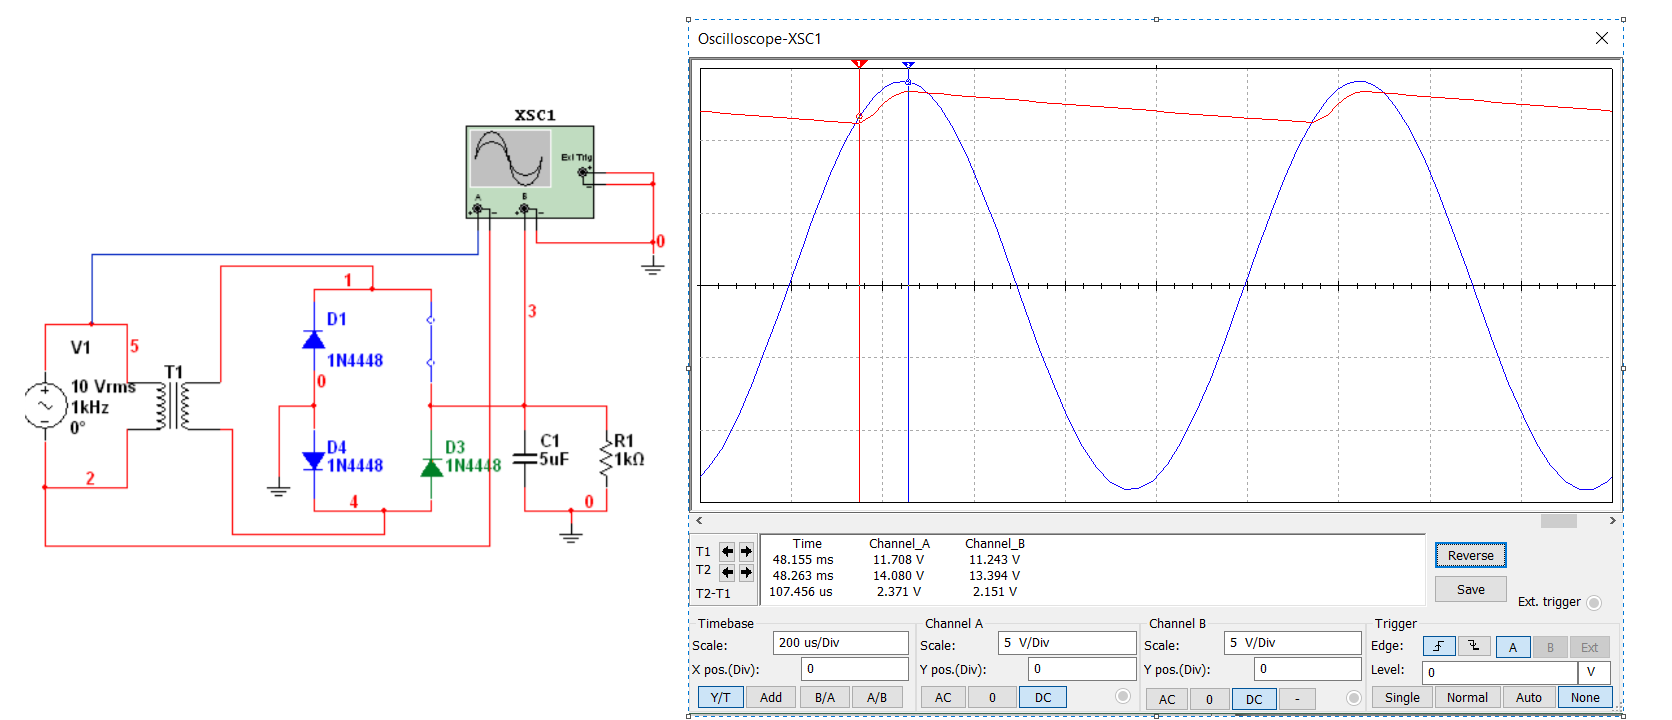
\includegraphics[width=10cm]{14}
\caption*{\textbf{Rys. 14}: Uszkodzenie diody w gałęzi mostka - wariant a.}
\end{figure}
\noindent W przypadku a) przebieg napięcia za prostownikiem jest taki sam jak dla prostownika jednopołówkowego.
\begin{figure}[H]
\centering
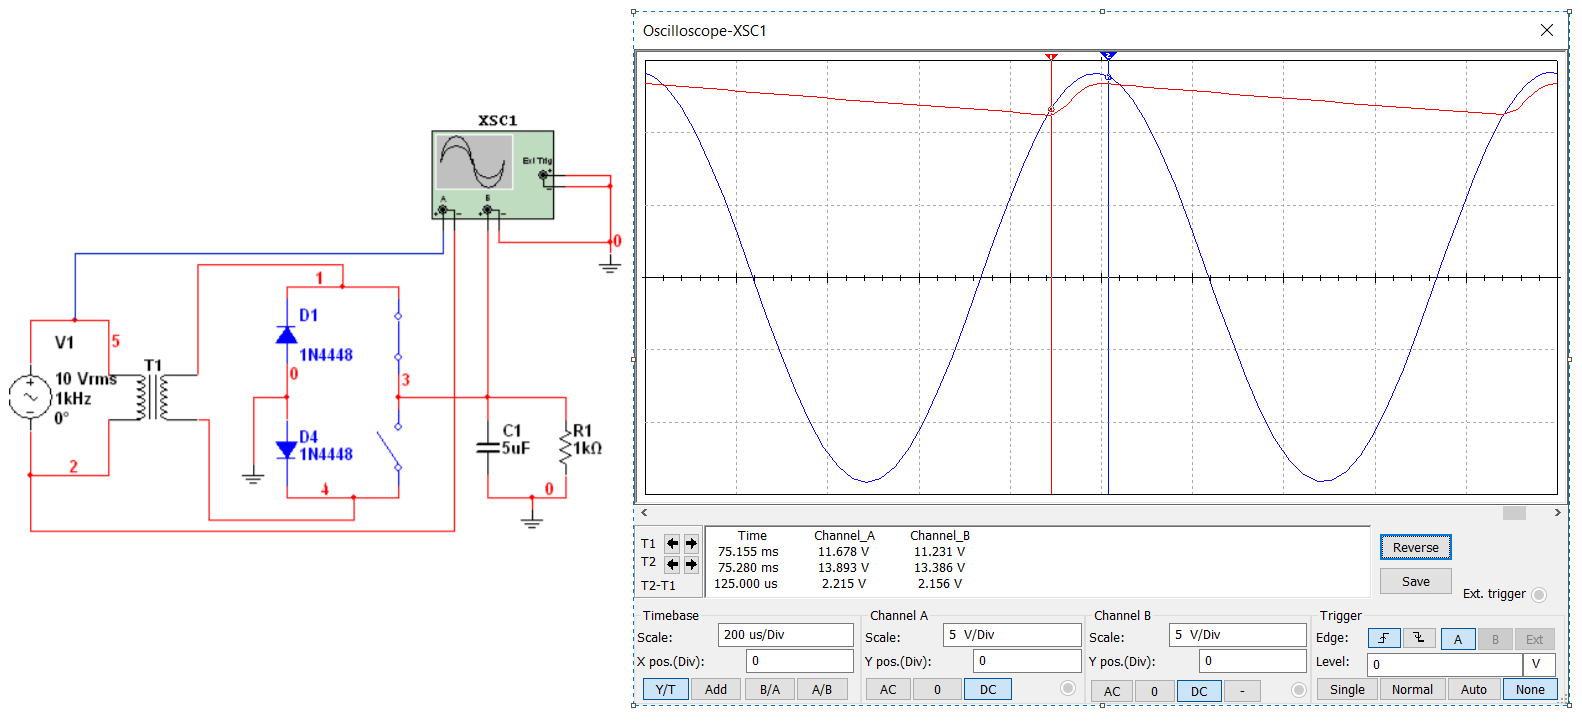
\includegraphics[width=10cm]{15}
\caption*{\textbf{Rys. 15}: Uszkodzenie diody w gałęzi mostka - wariant b.}
\end{figure}
\noindent W przypadku b) przebieg napięcia za prostownikiem jest również taki sam jak dla prostownika jednopołówkowego.
\begin{figure}[H]
\centering
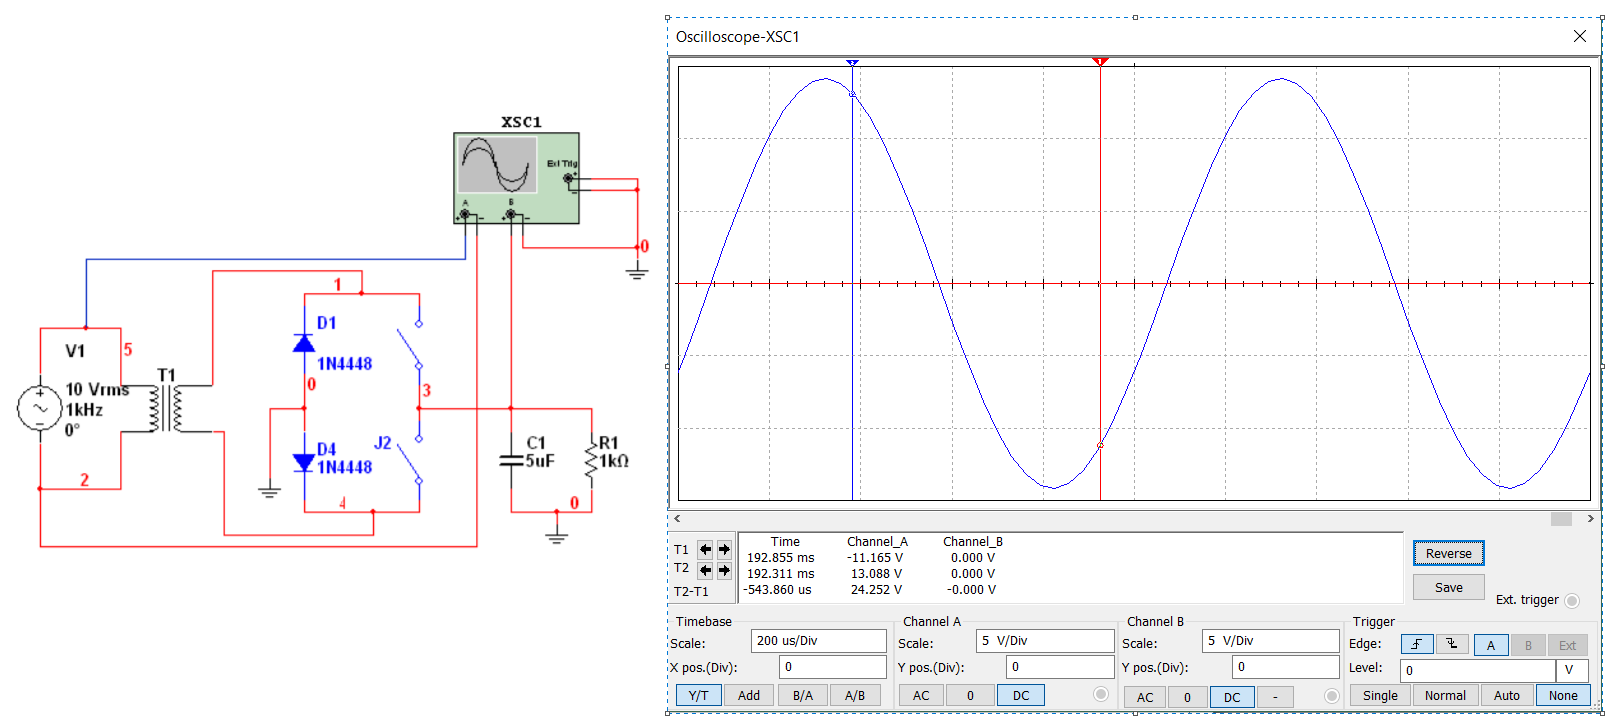
\includegraphics[width=10cm]{16}
\caption*{\textbf{Rys. 16}: Uszkodzenie diody w gałęzi mostka - wariant c.}
\end{figure}
\noindent W przypadku c) obwód jest otwarty więc napięcie za prostownikiem jest zawsze równe zero.
\subsection{Wnioski}
Prostownik w układzie Graetza działa w taki sam sposób jak prostownik jednopołówkowy, lecz wykorzystuje on również ujemną część przebiegu. Zachodzi to samo zjawisko co w poprzednim ćwiczeniu. Czym większa pojemność tym mniejsze tętnienia oraz czym większy opór tym mniejsze tętnienia (kondensator szybciej się 
ładuje). Możliwe uszkodzenia pokazały, że z owego układu można stworzyć prostownik jednopołówkowy (sytuacje a) i b)) lub prąd może nie płynąć w ogóle (sytuacja c)).
\section{Detektor szczytowy}
\subsection{Cel ćwiczenia}
Celem ćwiczenia było zapoznanie się z prostym detektorem szczytowym i przeanalizowanie jego działania.
\subsection{Przebieg ćwiczenia}
Detektor szczytowy wykorzystuje własności diody półprzewodnikowej i kondensatora. Napięcie na kondensatorze jest wprost proporcjonalne do zgromadzonego na nim ładunku elektrycznego. Dioda prostownicza umożliwia dopływ ładunku do kondensatora co sprawia, że ładunek kondensatora nie zmniejsza się.
Dopóki napięcie wejściowe obwodu detektora jest większe niż napięcie na kondensatorze to ładunek dopływa do kondensatora - dioda prostownicza jest wtedy spolaryzowana w kierunku przewodzenia. Dzieje się tak aż napięcie na kondensatorze zrówna się z napięciem wejściowym. Gdy napięcie na kondensatorze będzie
większe od wejściowego to dioda będzie spolaryzowana w kierunku zaporowym, a więc prąd w obwodzie nie będzie płynął, a ładunek na kondensatorze będzie stały. Umożliwia to pomiar największego dotychczas napięcia źródła. \newline
Na pulpicie symulacyjnym zbudowałem obwód elektryczny widoczny na \textbf{Rys. 17}. Przedstawiony poniżej układ zawiera źródło napięcia AM o wartości $V_1 = 5V$, diodę prostowniczą $D_1$ oraz kondensator o pojemności $6\mu$$F$. Do układu podłączyłem również oscyloskop w celu zbadania napięcia na kondensatorze.
\begin{figure}[H]
\centering
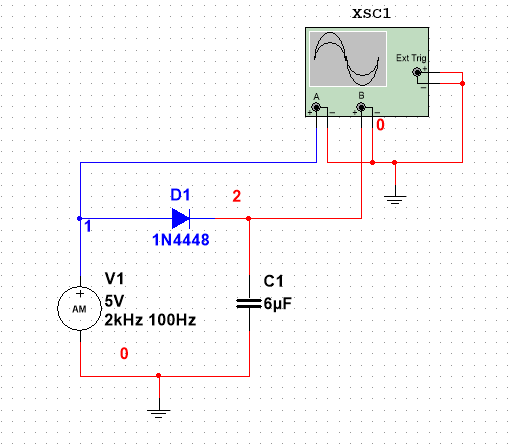
\includegraphics[width=10cm]{17}
\caption*{\textbf{Rys. 17}: Schemat detektora szczytowego. Układ zawiera również dołączony oscyloskop.}
\end{figure}
\noindent W celu zbadania napięcia na kondensatorze użyłem oscyloskopu oraz analizy Transient. Ekran oscyloskopu widać na \textbf{Rys. 18} zaś wyniki analizy Transient widoczne są na \textbf{Rys. 19}. W obu przypadkach napięcie na kondensatorze zaznaczone jest kolorem czerwonym zaś napięcie wejściowe - niebieskim.
\begin{figure}[H]
\centering
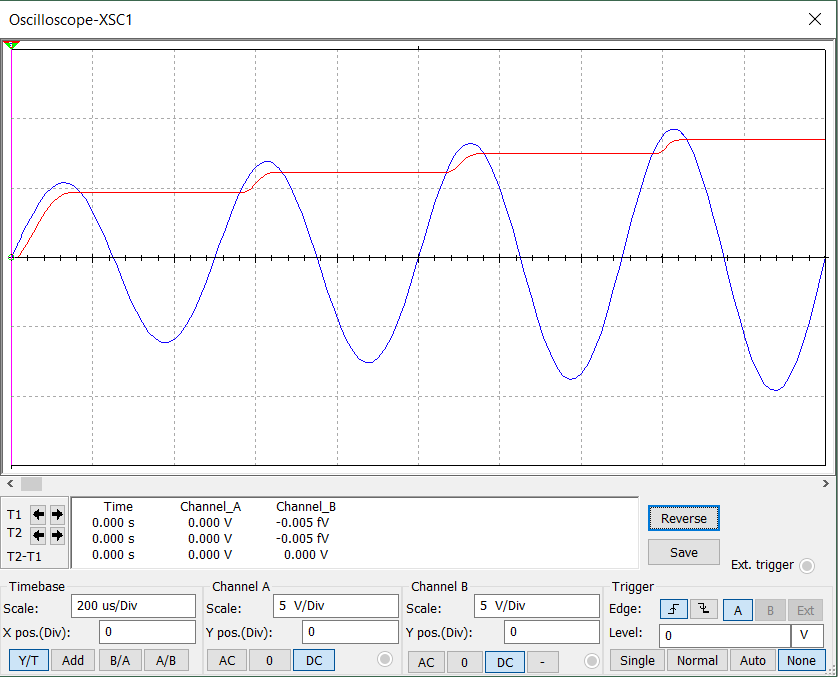
\includegraphics[width=10cm]{18}
\caption*{\textbf{Rys. 18}: Ekran oscyloskopu podłączonego do detektora szczytowego z Rys. 17}
\end{figure}
\begin{figure}[H]
\centering
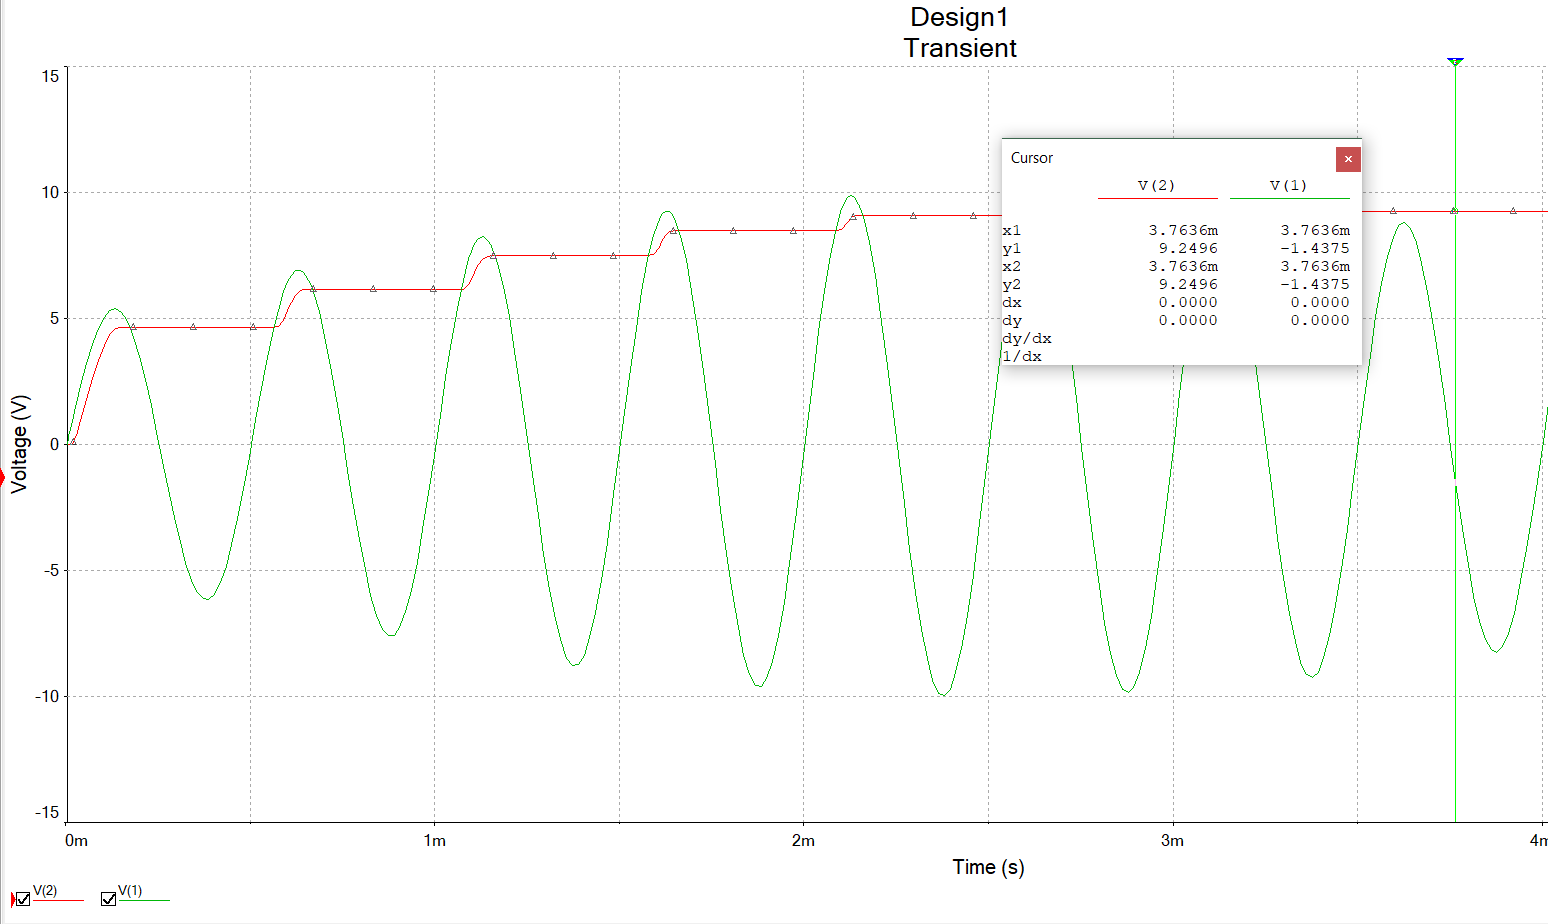
\includegraphics[width=10cm]{19}
\caption*{\textbf{Rys. 19}: Wyniki analizy Transient detektora szczytowego z  Rys. 17}
\end{figure}
\subsection{Wnioski}
Wyniki ćwiczenia pokazują, że detektor szczytowy działa prawidłowo. Napięcie na kondensatorze w danej chwili jest równe maksymalnemu do tej pory napięciu wejściowemu, pomniejszonemu o napięcie progowe diody półprzewodnikowej (ok. $0.7 V$). Zastosowanie dwóch metod pomiaru pozwoliło upewnić się co do 
poprawności obwodu.
\section{Demodulator diodowy}
\subsection{Cel ćwiczenia}
Celem ćwiczenia było zapoznanie się z prostym demodulatorem diodowym i zbadanie dla jakiej rezystancji obwód działa poprawnie.
\subsection{Przebieg ćwiczenia}
Układ demodulatora diodowego jest bardzo podobny do układu detektora szczytowego, z tą różnicą, że dodany został opornik. Układ ten ma na celu demodulację sygnału wejściowego, w którym kodowanie informacji oparte jest na zmianach w amplitudzie fali przenoszącej sygnał. Opornik rozładowuje kondensator
tak by ten odbierał kolejne maksymalne wartości sygnału na wejściu. W ten sposób otrzymuje się sygnał po demodulacji, czyli odkodowaną informację. \newline
Na pulpicie symulacyjnym zbudowałem obwód elektryczny widoczny na \textbf{Rys. 20}. Przedstawiony poniżej układ zawiera źródło napięcia AM o wartości $V_1 = 5V$, diodę prostowniczą $D_1$, kondensator o pojemności $10nF$ oraz opornik $R_1 = 1k\Omega$. Do układu podłączyłem również oscyloskop w celu
zbadania napięcia na kondensatorze.
\begin{figure}[H]
\centering
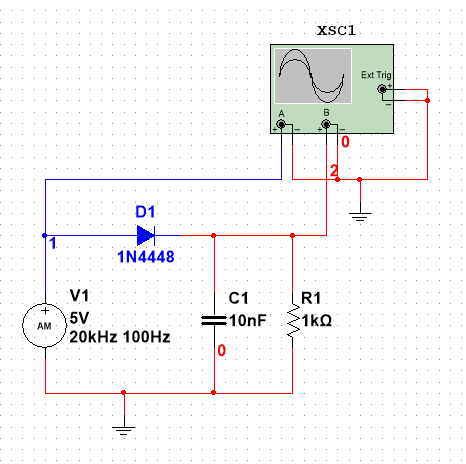
\includegraphics[width=10cm]{20}
\caption*{\textbf{Rys. 20}: Schemat demodulatora diodowego. Układ zawiera również dołączony oscyloskop.}
\end{figure}
\noindent Sprawdziłem działanie układu demodulatora diodowego na trzech różnych wartości rezystancji opornika. Na \textbf{Rys. 21}, \textbf{Rys. 22}, \textbf{Rys. 23} pokazałem odpowiedni układ i wyniki pomiarów oscyloskopu dla odpowiednio $R_1 = 1k\Omega$, $R_1 = 10k\Omega$, $R_1 = 100k\Omega$.
Na każdym rysunku napięcie na źródle jest zaznaczone kolorem niebieskim, napięcie na oporniku kolorem czerwonym. Jak widać, jedynie dla oporu $R_1 = 100k\Omega$ układ demodulatora działa prawidłowo, w innych przypadkach napięcie tętnień jest zbyt duże.
\begin{figure}[H]
\centering
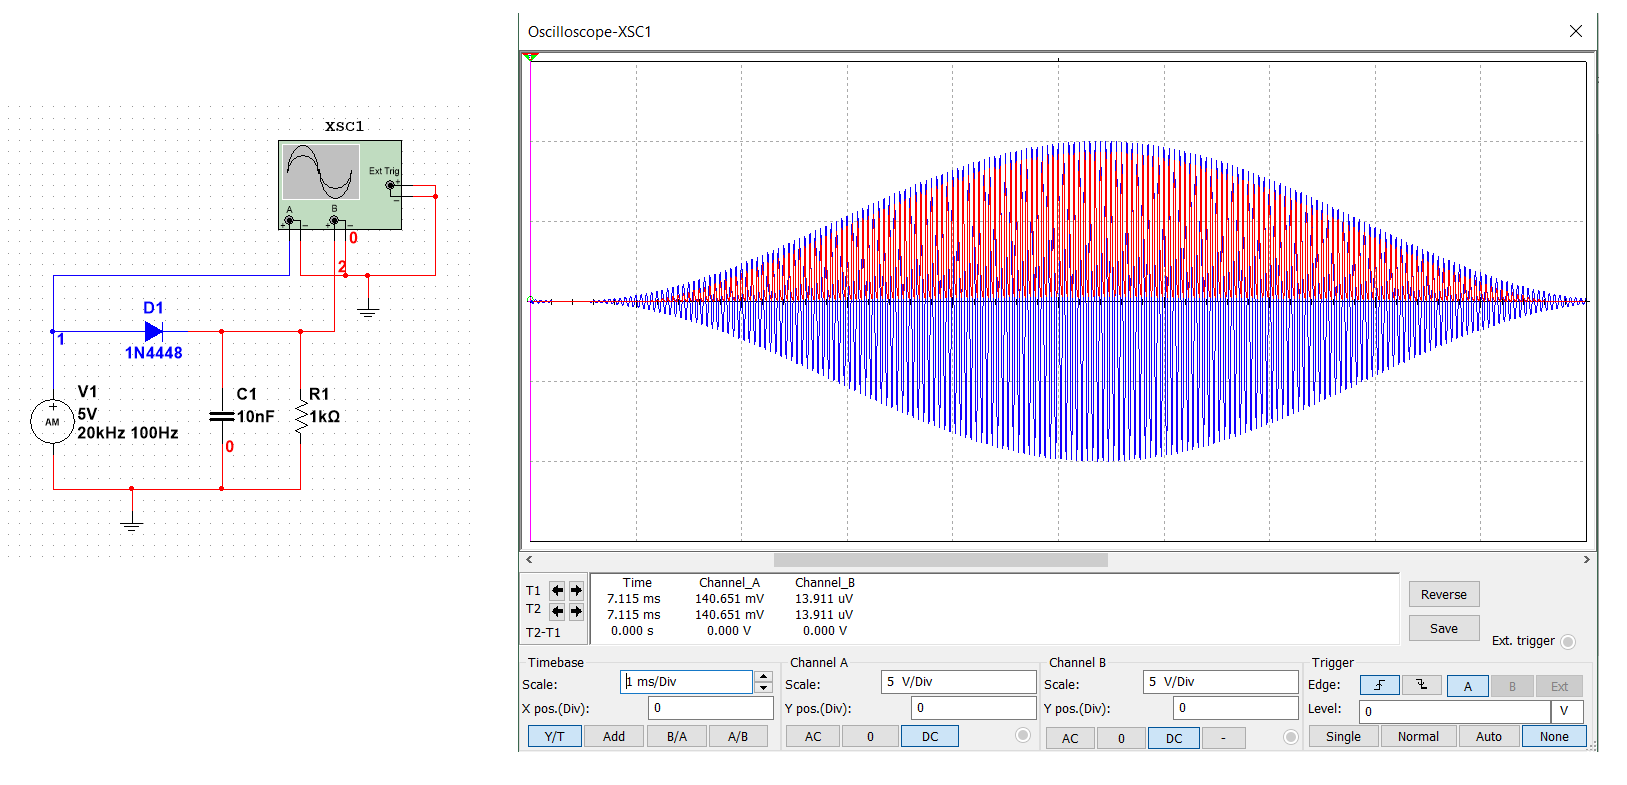
\includegraphics[width=10cm]{21}
\caption*{\textbf{Rys. 21}: Schemat demodulatora diodowego z oporem $R_1= 1k\Omega$. Obok układu pokazany ekran oscyloskopu. }
\end{figure}
\begin{figure}[H]
\centering
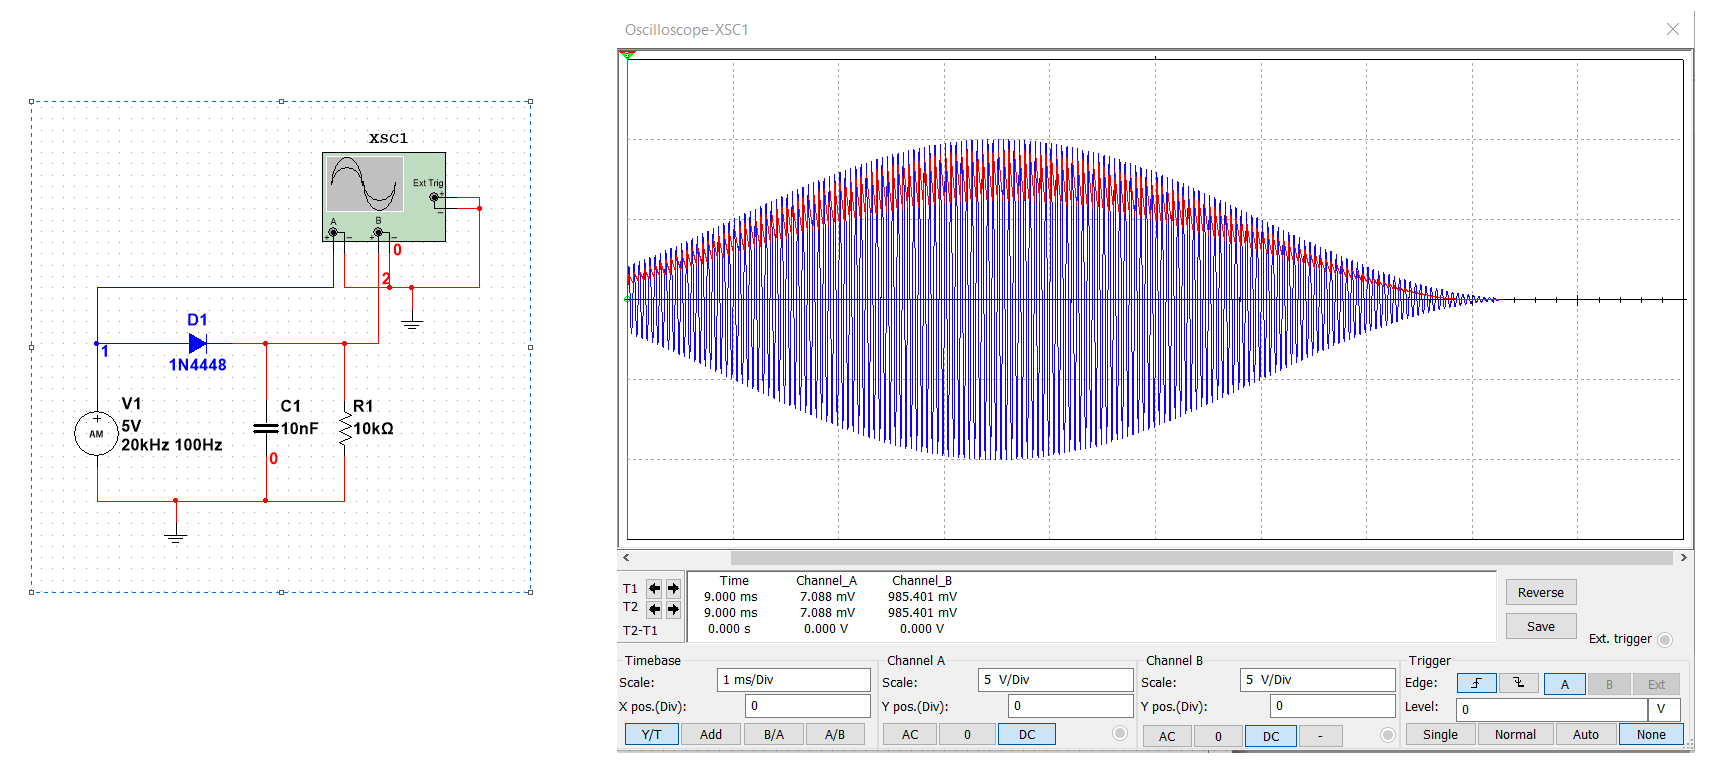
\includegraphics[width=10cm]{22}
\caption*{\textbf{Rys. 22}: Schemat demodulatora diodowego z oporem $R_1= 10k\Omega$. Obok układu pokazany ekran oscyloskopu. }
\end{figure}
\begin{figure}[H]
\centering
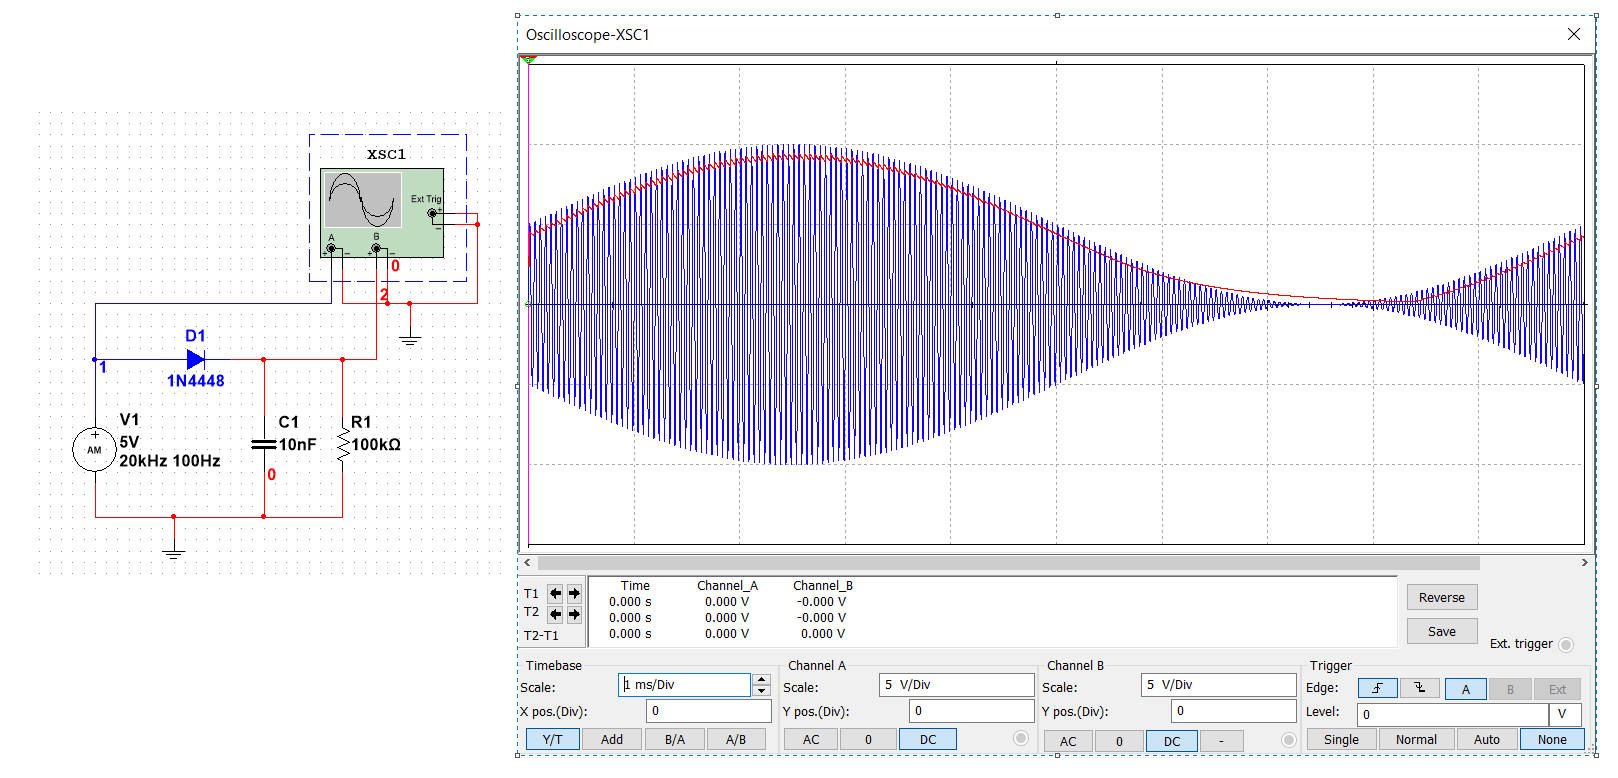
\includegraphics[width=10cm]{23}
\caption*{\textbf{Rys. 23}: Schemat demodulatora diodowego z oporem $R_1= 100k\Omega$. Obok układu pokazany ekran oscyloskopu. }
\end{figure}
\subsection{Wnioski}
Zbudowany układ demodulatora diodowego nie działał poprawnie dla rezystancji $1k\Omega$ i $10k\Omega$ ponieważ napięcie tętnień było zbyt duże. Poprawne działanie demodulatora udało się uzyskać dopiero dla oporu $100k\Omega$. Przebieg napięcia na oporniku był wtedy zbliżony do sygnału źródłowego (modulującego) 
pomniejszonego o napięcie progowe diody półprzewodnikowej. Widać więc, że dla odpowiedniej wartości można użyć układu demodulatora diodowego do zmierzenia napięcia progowego diody.
\section{Ogranicznik diodowy}
\subsection{Cel ćwiczenia}
Celem ćwiczenia było zapoznanie się z układami ogranicznika diodowego z użyciem diody półprzewodnikowej oraz źródła stałego napięcia.
\subsection{Przebieg ćwiczenia}
Na pulpicie symulacyjnym zbudowałem kilka wersji obwodu ogranicznika diodowego. Obwody różniły się liczbą zastosowanych diód, kierunkiem przewodzenia oraz obecności dodatkowego źródła napięcia polaryzującego. Każdy z obwodów składał się ze źródła napięcia zmiennego $V_1 = 10V$, diód półprzewodnikowych
$D_1$ ($D_2$, $D_3$), oraz dwóch oporników o wartościach rezystancji $5k\Omega$, jednego podłączonego szeregowo do diody, drugiego równolegle. Do układów podłączyłem również oscyloskop w celu zbadania napięcia na wejściu i wyjściu układu. Na ekranie oscyloskopu obserwowalem przebieg napięcia wejściowego i 
napięcia wyjściowego układu. Odpowiednie układy i ekrany oscyloskopów widać na \textbf{Rys. 24},\textbf{Rys. 25},\textbf{Rys. 26},\textbf{Rys. 27},\textbf{Rys. 28},\textbf{Rys. 29}.
\begin{figure}[H]
\centering
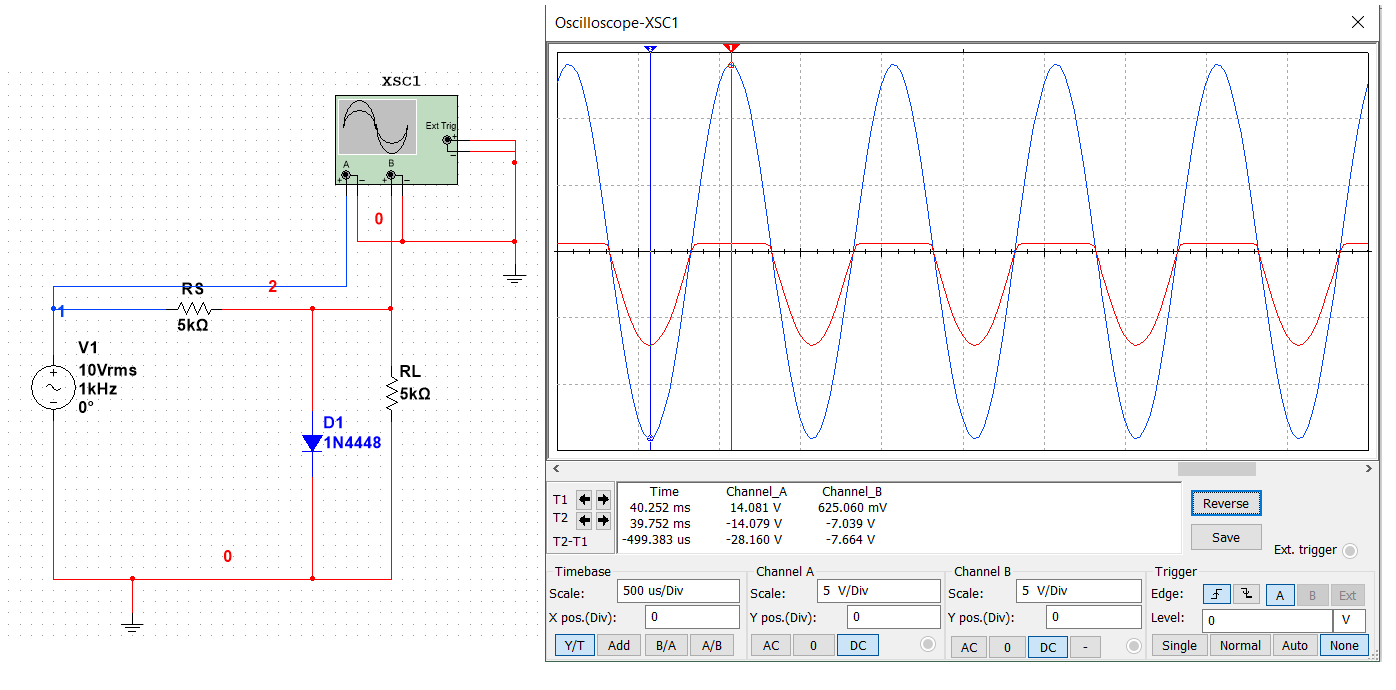
\includegraphics[width=10cm]{24}
\caption*{\textbf{Rys. 24}: Schemat ogranicznika diodowego z jedną diodą - wersja 1. Obok układu pokazany ekran oscyloskopu. }
\end{figure}
\begin{figure}[H]
\centering
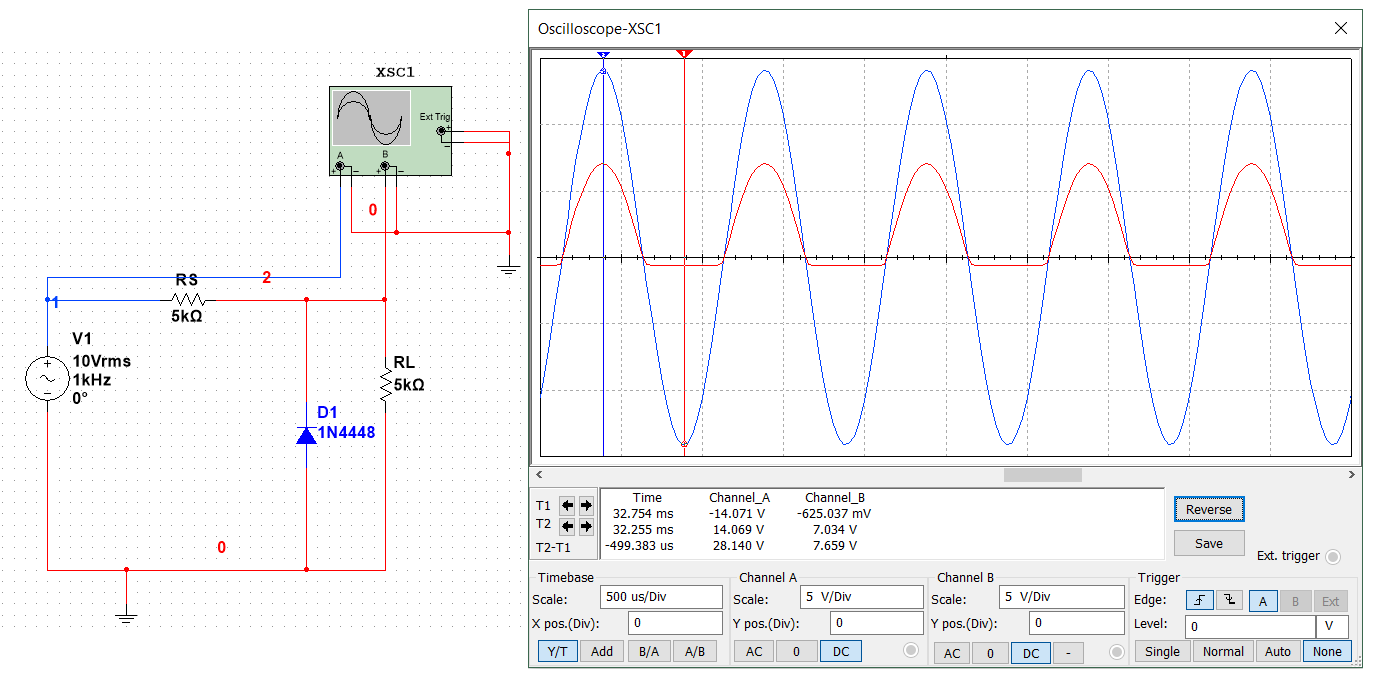
\includegraphics[width=10cm]{25}
\caption*{\textbf{Rys. 25}: Schemat ogranicznika diodowego z jedną diodą - wersja 2. Obok układu pokazany ekran oscyloskopu. }
\end{figure}
\begin{figure}[H]
\centering
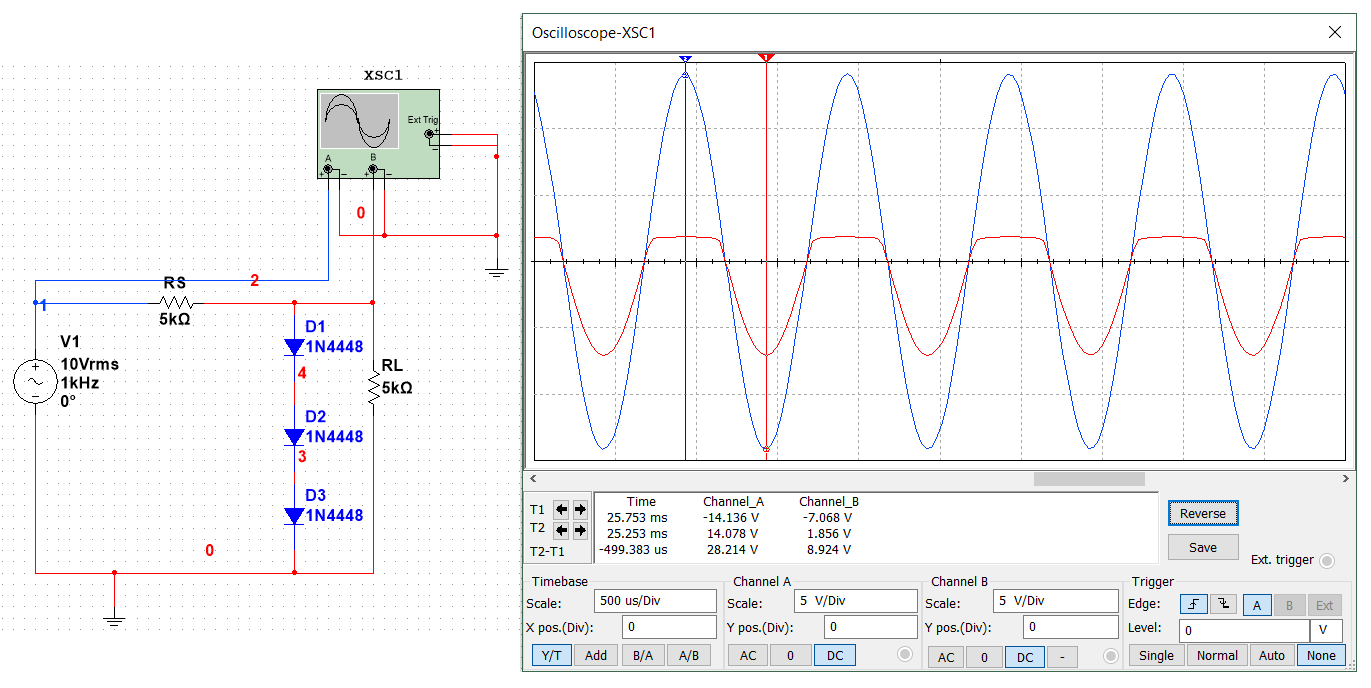
\includegraphics[width=10cm]{26}
\caption*{\textbf{Rys. 26}: Schemat ogranicznika diodowego z trzema diodami. Obok układu pokazany ekran oscyloskopu. }
\end{figure}
\begin{figure}[H]
\centering
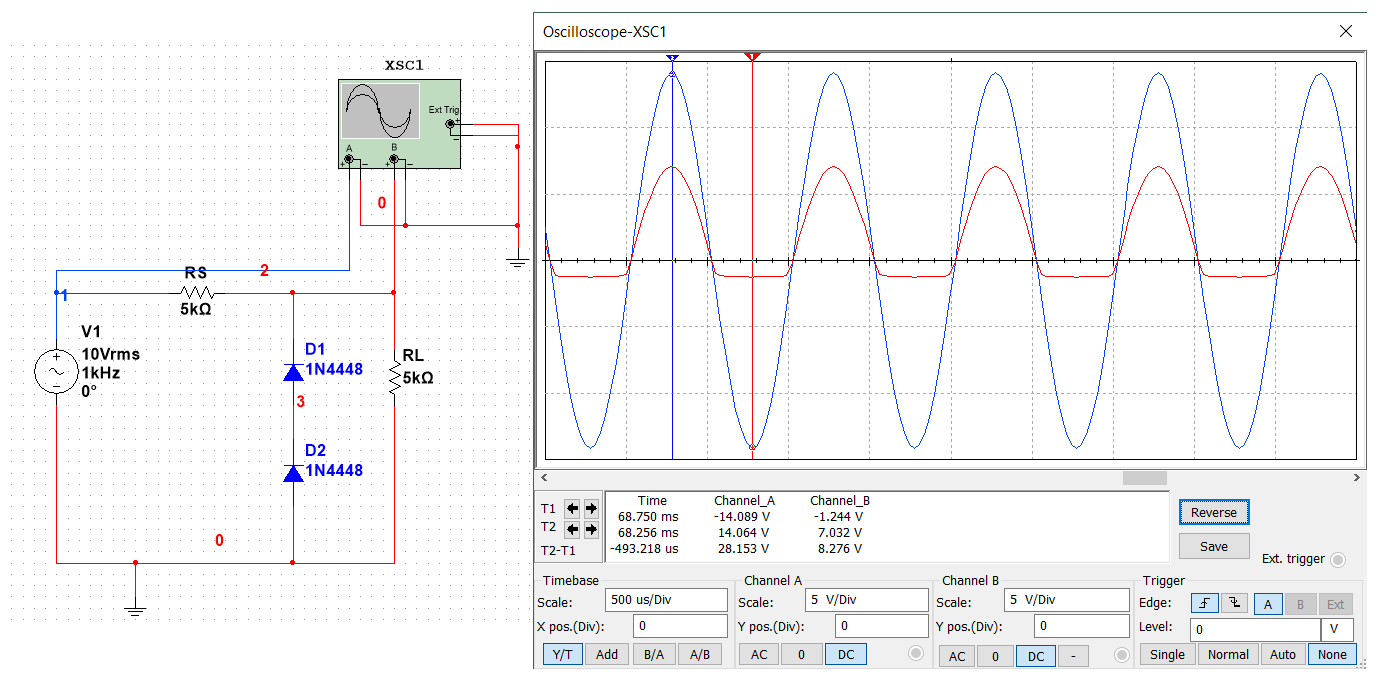
\includegraphics[width=10cm]{27}
\caption*{\textbf{Rys. 27}: Schemat ogranicznika diodowego z dwoma diodami. Obok układu pokazany ekran oscyloskopu. }
\end{figure}
\begin{figure}[H]
\centering
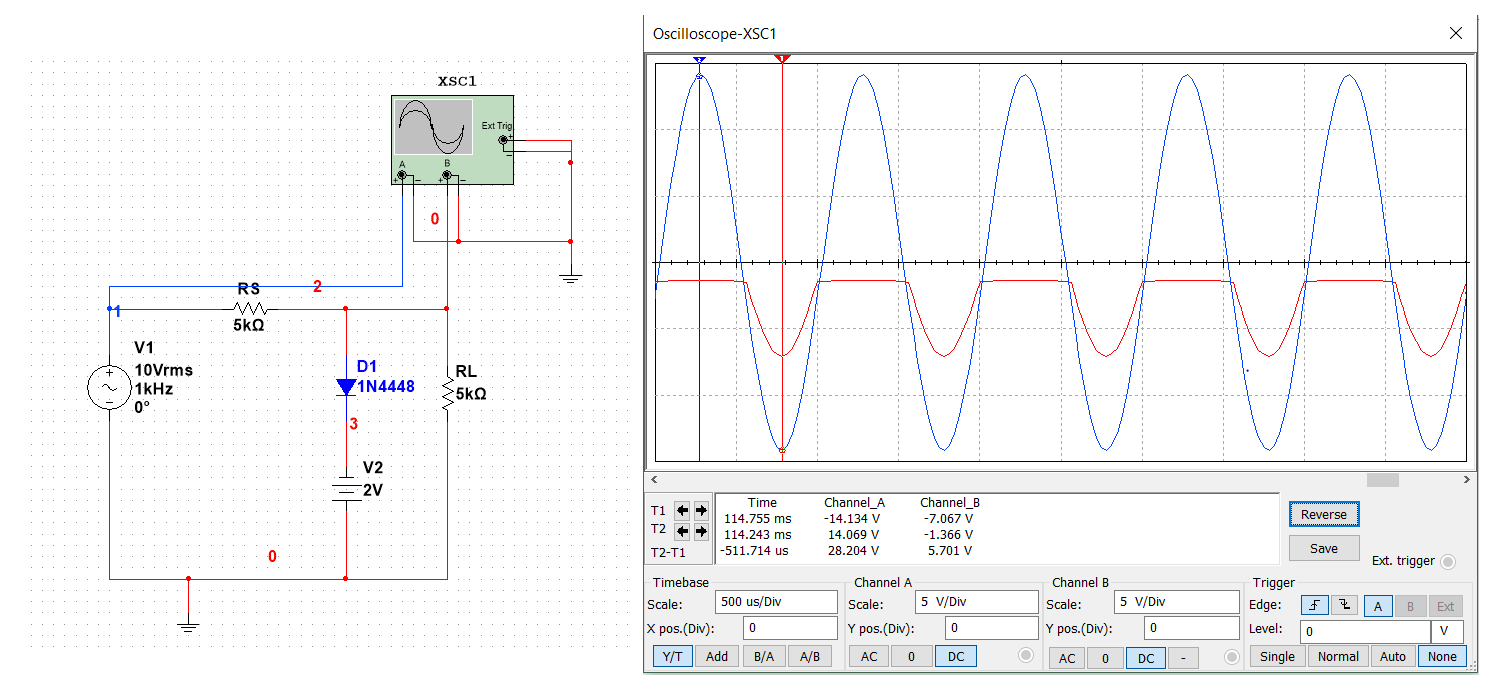
\includegraphics[width=10cm]{28}
\caption*{\textbf{Rys. 28}: Schemat ogranicznika diodowego z diodą i dodatkowym źródłem napięcia polaryzującego - wersja 1. Obok układu pokazany ekran oscyloskopu. }
\end{figure}
\begin{figure}[H]
\centering
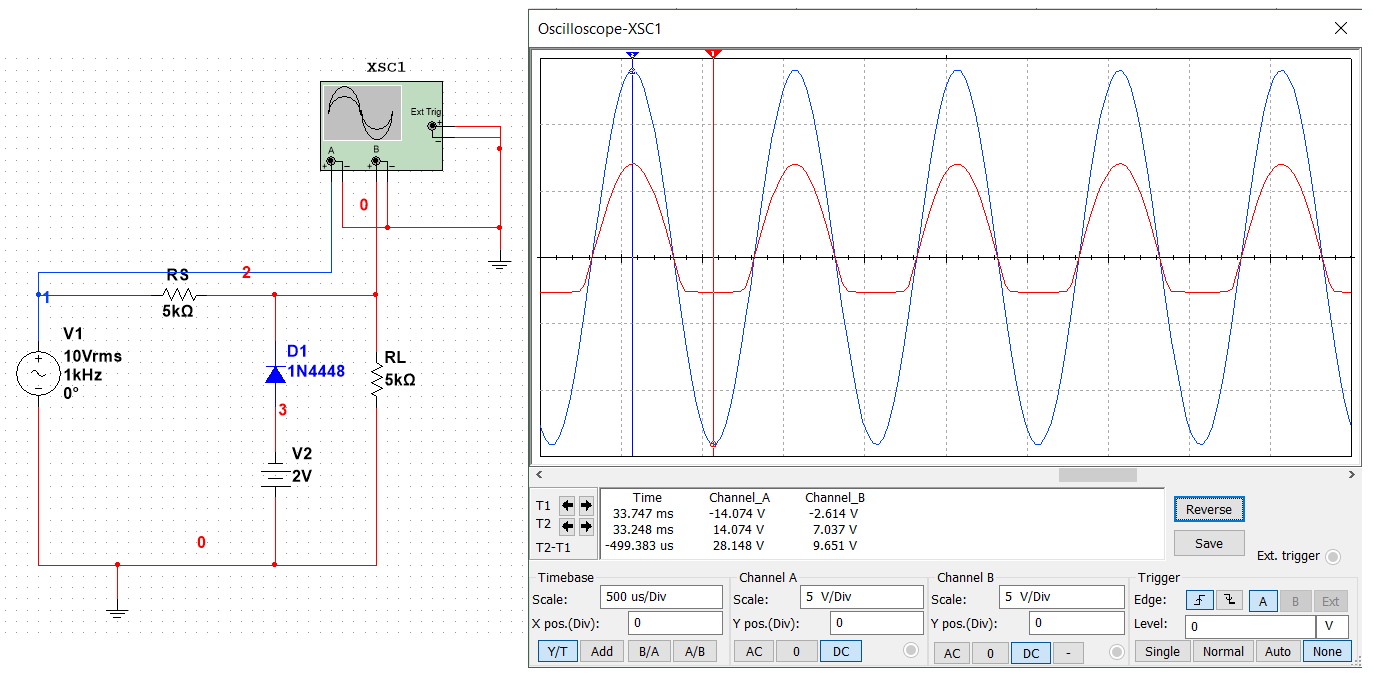
\includegraphics[width=10cm]{29}
\caption*{\textbf{Rys. 29}: Schemat ogranicznika diodowego z diodą i dodatkowym źródłem napięcia polaryzującego - wersja 2. Obok układu pokazany ekran oscyloskopu. }
\end{figure}
\subsection{Wnioski}
Pokazane układy diód prostowniczych oraz źródeł napięcia polaryzującego służą do ograniczania napięcia na wyjściu układu dla obu biegunowości. Przy dobraniu odpowiednich parametrów obwodu (liczba diód półprzewodnikowych, ich kierunek przewodzenia, obecność dodatkowego źródła napięcia) możliwe jest
uzyskanie przebiegu, którego jedna część ma charakter sinusoidalny, a druga ma charakter napięcia stałego.
\end{document}